\documentclass{beamer}
 
\usepackage[utf8]{inputenc}
\usepackage[english,russian]{babel}
\usepackage{graphicx}
\graphicspath{ {./pictures/} }
\usepackage{color}


\mode<presentation> {\usetheme{default}}
\setbeamertemplate{itemize items}[triangle]
 
\title[Distributed map-reduce]{Курсовой проект \\ \it{Фреймворк и файловая система для распределённой обработки больших данных в рамках концепции map-reduce}}

\author{Выборнов А.И.} % Your name
\institute[МГТУ ИУ-9] {
    МГТУ~им.~Н.~Э.~Баумана \\
    \medskip
    \text{art-vybor@ya.com}
}
\date{\today}

\begin{document}
%----------------------------------------------------------------------------------------
%    Title
%----------------------------------------------------------------------------------------
\begin{frame}
    \titlepage
\end{frame}

%----------------------------------------------------------------------------------------
%   Revierw
%----------------------------------------------------------------------------------------

\begin{frame}
\frametitle{Обзор} 
\tableofcontents 
\end{frame}

%----------------------------------------------------------------------------------------
%   Presentation
%----------------------------------------------------------------------------------------

\section{Постановка задачи}
    \begin{frame}
    \frametitle{Постановка задачи}
        \begin{itemize}
            \item Анализ требований и проектирование архитектуры системы. Реализация нераспределённого map-reduce. Решение проблемы RPC.
            \item Реализация распределённой файловой системы. Реализация фреймворка. Тестирование на примерах.
            
        \end{itemize} 
    \end{frame}

\section{Концепция map-reduce}
    \begin{frame}
    \frametitle{Зачем нужен map-reduce?}
        \begin{itemize}
            \item Обработка больших данных (Big Data).
            \begin{itemize}
                \item Вычисления превосходят возможности одной машины.  
                \item Данные не помещаются в памяти, необходимо обращаться к диску.
                \item Можно хранить много данных, но задержки и пропускная способность оборудования растут пропорционально данным.
            \end{itemize}
            \item Удобная абстракция для построения алгоритмов обработки больших данных.
            \item Устойчивость к отказам.            
        \end{itemize} 
    \end{frame}

    \begin{frame}
    \frametitle{Что такое map-reduce?}
        \begin{itemize}
            \item Структура (key, value) - пара (ключ, значение).
            \item Программирование представляет собой определение двух функций:
            \begin{itemize}
                \item $map: (key, value)\rightarrow[(key, value)]$
                \item $reduce: (key, [value])\rightarrow[(key, value)]$
            \end{itemize}
            \item Между стадиями $map$ и $reduce$ происходит группировка и сортировка данных.
            
        \end{itemize} 
    \end{frame}

    \begin{frame}
    \frametitle{Map-reduce на примере - Поиск общих друзей}
        \begin{itemize}
            \item {\bfЗадача:} Есть граф пользователей некоторого ресурса, заданный в виде строчек: <<пользователь - друг1 друг2 ...>>. Для каждой пары пользователей найти общих друзей.
            \item Разберём задачу на следующих входных данных: \\
                \begin{itemize}
                    \item A - B C D
                    \item B - A C
                    \item C - A B D
                    \item D - A C
                \end{itemize}          
        \end{itemize} 
    \end{frame}  


    \begin{frame}
    \frametitle{Map-reduce на примере - Поиск общих друзей}
        \begin{itemize}
            \item На стадии map преобразовываем пару (пользователь, друзья) в множество пар следующим образом:
            \begin{itemize}
                \item (A, B C D) -> (A B, B C D), (A C, B C D), (A D, B C D)
                \item (B, A C) -> (A B, A C), (B C, A C)
                \item (C, A B D) -> (A C, A B D), (B C, A B D), (C D, A B D)
                \item (D, A C) -> (A D, A C), (C D, A C)
            \end{itemize}
        \end{itemize}
    \end{frame} 

    \begin{frame}
    \frametitle{Map-reduce на примере - Поиск общих друзей}
        \begin{itemize}
            \item Сливаем результаты полученные на стадии map, получаем список пар:
            \begin{itemize}
                \item (A B, [B C D, A C])
                \item (A C, [B C D, A B D])
                \item (A D, [B C D, A C])
                \item (B C, [A B D, A C])
                \item (C D, [A B D, A C])
            \end{itemize}
        \end{itemize}
    \end{frame} 

    \begin{frame}
    \frametitle{Map-reduce на примере - Поиск общих друзей}
        \begin{itemize}
            \item На стадии reduce пересекаем с друг другом все элементы списка значений и получаем:
            \begin{itemize}
                \item (A B, C)
                \item (A C, B D)
                \item (A D, C)
                \item (B C, A)
                \item (C D, A)
            \end{itemize}
        \end{itemize}
    \end{frame} 

\section{Архитектура}

    \begin{frame}
    \frametitle{Архитектура распределённого map-reduce}
        \begin{figure}[h!]
            \begin{center}
                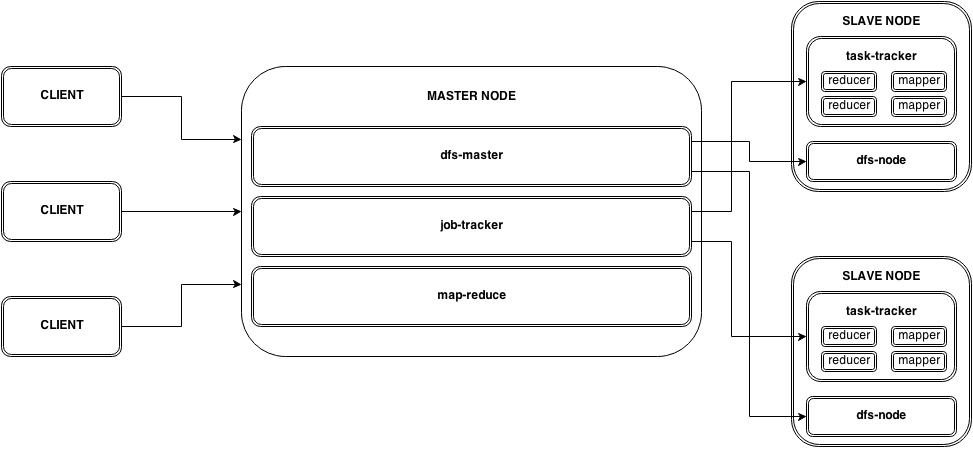
\includegraphics[scale=0.5]{map-reduce.png}
            \end{center}
        \end{figure}        
    \end{frame}


    \begin{frame}
    \frametitle{Как работает распределённая файловая система}
        \begin{itemize}
            \item Файл разбивается на блоки фиксированного размера (64мб).
            \item Получившиеся блоки распределяются по машинам.
            \item Cтруктура фс - дерево, в котором узлы соответствуют папкам, а листья - файлам.
            \item Файл представляет собой список индексов.
            \item BlockManager - класс, раздающий новых индексы и содержащий таблицу отображения блоков в конкретную ноду.
        \end{itemize}
    \end{frame}



    \begin{frame}
    \frametitle{Как работает распределённый map-reduce}
        \begin{itemize}
            \item На вход подаются адреса файлов в DFS для ввода и вывода, а также файл с функциями map и reduce.
            \item Стадии выполнения:
            \begin{itemize}
                \item Получение по входному файлу списка индексов в DFS.
                \item Разбиение списка индексов по узлам.
                \item Выполнение стадии map на узлах.
                \item Распределение данных между узлами.
                \item Выполнение стадии reduce на узлах.
                \item Добавление результатов функций reduce в виде файла в DFS.
                \begin{itemize}
                    \item Переименование результатов.
                    \item Запись информации о новом файле в DFS.
                \end{itemize} 
            \end{itemize} 
        \end{itemize}        
    \end{frame}

    \begin{frame}
    \frametitle{Архитектура распределённого map-reduce}
        \begin{figure}[h!]
            \begin{center}
                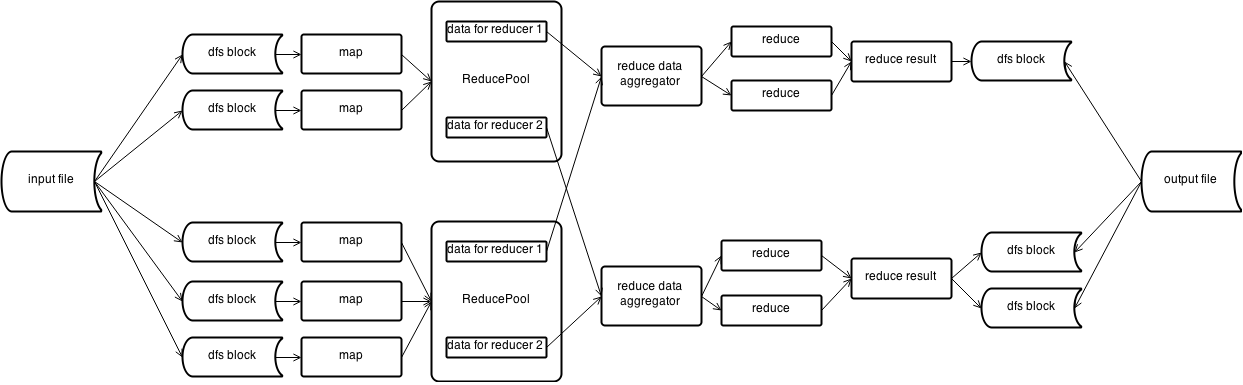
\includegraphics[scale=1]{total_data.png}
            \end{center}
        \end{figure}        
    \end{frame}


    \begin{frame}
    \frametitle{Как работает map на узлах}
        \begin{itemize}
            \item По списку индексов получаются данные путём обращения к узлу dfs, находящемуся на этой машине.
            \item Для каждого индекса выполняется переданная функция map.
            \item Результаты каждого map в виде ассоциативного массива передаются структуре reduce pool.
            \item По окончании оставшиеся в reduce pool данные отправляются по узлам.
        \end{itemize}        
    \end{frame}

    \begin{frame}
    \frametitle{Как работает reduce на узлах}

        \begin{itemize}
            \item Cливает результаты стадий map и распределяет их по узлам.
            \item Cтруктура reduce pool состоит из набора ассоциативных массивов, каждый из которых соответствует одному slave узлу.
            \item Данные переданные в структуру reduce pool равномерно распределяются среди набора массивов.
            \item После добавления новых данных структура проверяет, не превышает ли один элементов набора установленного размера. При превышении установленного размера элемент отправляется на соответсвующий узел. 
            \item На узлах, все полученные от reduce pool данные аккумулируются.
        \end{itemize}        
    \end{frame}


    \begin{frame}
    \frametitle{Как работает reduce на узлах}
        \begin{itemize}
            \item Разбивает все данные на блоки пар, по возможности, не превышающие фиксированного размера с точность до одной пары.
            \item Для каждой полученный пары выполняется переданная функция reduce.
            \item Полученный результат разбивается на блоки равного размера (64мб).
            \item Блоки записываются в dfs на узел, где выполнялся reduce под псевдоименами.
        \end{itemize}        
    \end{frame}


\section{Отчёт}
    \begin{frame}
    \frametitle{Что сделано}
        \begin{itemize}
            \item Разработаны архитектуры распределённых map-reduce и файловой системы.
            \item Реализован распределённый map-reduce.
            \item Для реализации RPC была выбрана связка: ZeroMQ + Marshal.
            \item Реализована распределённая файловая система для хранения больших данных.
        \end{itemize} 
    \end{frame}

    \begin{frame}
    \frametitle{Что не реализовано}
        \begin{itemize}            
            \item Существует узкое место при аггрегации данных перед стадией reduce (reduce pool) - возможно переполнение оперативной памяти. Исправить можно следующим образом:
            \begin{itemize}
                \item При получении данных, они добавляются в ассоциативный массив.
                \item При превышении массивом установленного размера он сортируется и выгружается на диск.
                \item Перед выполнением стадии reduce необходимо отсортировать и выгрузить на диск оставшиеся в массиве данные.
                \item Во время выполнения стадии reduce полученные файлы на лету сливаются и обрабатываются функцией reduce.
            \end{itemize} 
        \end{itemize} 
    \end{frame}

    \begin{frame}
    \frametitle{Что предстоит сделать}
        \begin{itemize}
            \item Подготовить код распределённого map-reduce для тестов.
            \item Протестировать полученную систему на больших данных и проанализировать результаты.
        \end{itemize} 
    \end{frame}

\begin{frame}
    \titlepage
\end{frame}

\end{document}